\documentclass[letterpaper,12pt,fleqn]{article}
\usepackage{matharticle}
\usepackage{siunitx}
\usepackage{graphicx}
\pagestyle{plain}
\newcommand{\dT}{\Delta T}
\begin{document}

\begin{center}
  \large
  Math-19 Section 1

  \Large
  Homework \#3 Solutions
\end{center}

\subsection*{Problems}

\begin{enumerate}
\item The amount of heat energy (\(Q\)) needed to change the temperature of an object (without going through a
  phase change like melting or boiling) is jointly proportional to the mass of the object (\(m\)) and the
  \emph{change} in temperature (\(\dT\)).
\begin{enumerate}
\item Write an equation that models this physical phenomenon. Use $c$ for the constant of proportionality.
  \[Q=cm\dT\]
\item The MKS unit for heat energy is the Joule (\(J\)). The constant of proportionality is specific to the
  substance being heated and is referred to as the \emph{specific heat} of the substance. If \(Q\) is measured in
  Joules (\(J\)), \(m\) is measured in grams (\(g\)), and temperature is measured in Kelvin (\(K\)), what are the
  units of \(c\)?
  \begin{gather*}
    J=\left(\frac{J}{gK}\right)gK
  \end{gather*}
\item In the lab, it is found that \SI{41790}{J} of heat energy raises the temperature of \SI{1}{L} of water by
  \SI{10}{K}. What is the specific heat of water?  (\SI{1}{L} of water=\SI{1000}{g})
  \[c=\frac{J}{m\dT}=\frac{41790}{1000\cdot10}=\SI{4.1790}{J/gK}\]
\end{enumerate}

\item Consider the equation:
  \[y=x^2+2x-5\]
  For each of the parts below, use the graphing functions from your TI-84 \emph{calc} menu to find the answers and
  submit a screen-shot from your calculator that shows the correct answer.
  \begin{enumerate}
  \item Find the \(y\)-value when \(x=1.3\) using the \emph{value} function.
    
    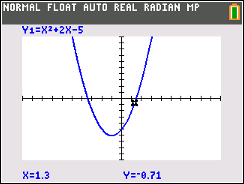
\includegraphics[scale=0.75]{hw3-2a}
    
  \item Find the \(x\)-intercepts using the \emph{zero} function.

    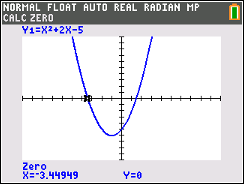
\includegraphics[scale=0.75]{hw3-2b1}\hspace{0.25in}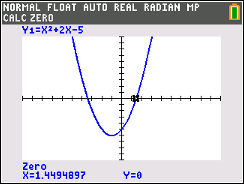
\includegraphics[scale=0.75]{hw3-2b2}

  \item Determine the minimum value using the \emph{minimum} function.
    
    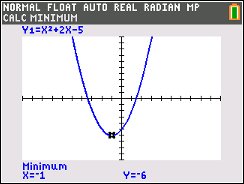
\includegraphics[scale=0.75]{hw3-2c}
    
  \item Determine the \(x\)-values for \(y=5\) using the \emph{intersect} function.  Note that you will need to add
    something to your graph to do this. Also note that there are multiple answers.
    
    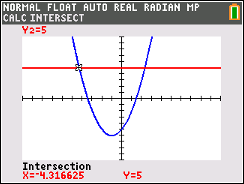
\includegraphics[scale=0.75]{hw3-2d1}\hspace{0.25in}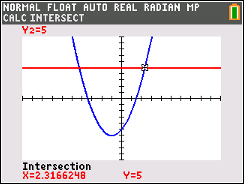
\includegraphics[scale=0.75]{hw3-2d2}
    
  \item Now graph the function \(y=x^2+11\). Huh!? Nothing seems to appear! Why, and how can you fix this? Submit a
    screen shot that uses your fix.

    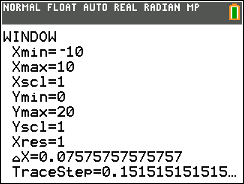
\includegraphics[scale=0.75]{hw3-2e1}\hspace{0.25in}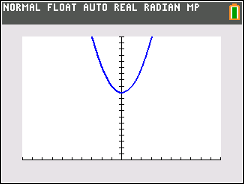
\includegraphics[scale=0.75]{hw3-2e2}
  \end{enumerate}
\end{enumerate}

\end{document}
